%%%%%%%%%%%%%%%%%%%%%%%%%%%%%%%%%%%%%%%%%%%%%%%%%%%%%%%%%%%%
% 3.9 COMPLEX GEOMETRY
% The Composition of Advanced Mathematics
%%%%%%%%%%%%%%%%%%%%%%%%%%%%%%%%%%%%%%%%%%%%%%%%%%%%%%%%%%%%

\section{Complex Geometry}
\label{sec:complex-geometry}

\prerequisite{
Complex numbers and functions, Multivariable Calculus, Linear Algebra,
Topology, Differential Geometry from \cref{sec:differential-geometry},
and Algebraic Geometry from \cref{sec:algebraic-geometry}.
}

\learningobjectives{
By the end of this section, the reader should be able to:
\begin{itemize}
    \item explain the basic goals of complex geometry;
    \item distinguish real and complex dimensions;
    \item describe complex manifolds using holomorphic coordinate charts;
    \item explain holomorphic transition maps;
    \item recognize Riemann surfaces as complex one-dimensional manifolds;
    \item work with complex tangent spaces and complex coordinates;
    \item distinguish holomorphic, Hermitian, and K\"ahler structures;
    \item explain the role of complex differential forms;
    \item distinguish forms of type \((p,q)\);
    \item describe the operators \(\partial\) and \(\bar{\partial}\);
    \item explain Hermitian metrics and their associated fundamental forms;
    \item state the defining condition for a K\"ahler manifold;
    \item recognize basic examples of complex manifolds;
    \item explain complex projective space as a complex manifold;
    \item describe complex tori and complex curves;
    \item explain the relationship between complex geometry and algebraic geometry;
    \item recognize the roles of divisors, line bundles, and the canonical bundle;
    \item explain the broad significance of Hodge theory;
    \item identify major applications of complex geometry.
\end{itemize}
}

%%%%%%%%%%%%%%%%%%%%%%%%%%%%%%%%%%%%%%%%%%%%%%%%%%%%%%%%%%%%
\subsection{What Is Complex Geometry?}
\label{subsec:what-is-complex-geometry}
%%%%%%%%%%%%%%%%%%%%%%%%%%%%%%%%%%%%%%%%%%%%%%%%%%%%%%%%%%%%

Complex geometry studies geometric spaces whose local coordinates are
complex numbers and whose coordinate changes are holomorphic.

The basic local model is

\[
\boxed{\C^n.}
\]

A point in \(\C^n\) has coordinates

\[
(z_1,\ldots,z_n),
\]

where each

\[
z_j=x_j+iy_j.
\]

Thus complex geometry combines ideas from

\[
\boxed{
\text{geometry}
+
\text{topology}
+
\text{complex analysis}.
}
\]

\begin{definitionbox}{Complex Geometry}
\emph{Complex geometry} is the study of geometric spaces equipped with
complex-analytic structures, particularly complex manifolds and geometric
structures compatible with them.
\end{definitionbox}

%%%%%%%%%%%%%%%%%%%%%%%%%%%%%%%%%%%%%%%%%%%%%%%%%%%%%%%%%%%%
\subsection{Complex Coordinates}
\label{subsec:complex-coordinates}
%%%%%%%%%%%%%%%%%%%%%%%%%%%%%%%%%%%%%%%%%%%%%%%%%%%%%%%%%%%%

A complex coordinate has the form

\[
\boxed{z=x+iy,}
\]

where

\[
i^2=-1.
\]

Its complex conjugate is

\[
\boxed{\bar z=x-iy.}
\]

The notation

\[
\bar z
\]

is read ``z bar'' or ``the complex conjugate of \(z\).''

We can recover the real coordinates using

\[
\boxed{x=\frac{z+\bar z}{2}}
\]

and

\[
\boxed{y=\frac{z-\bar z}{2i}.}
\]

%%%%%%%%%%%%%%%%%%%%%%%%%%%%%%%%%%%%%%%%%%%%%%%%%%%%%%%%%%%%
\subsection{Real and Complex Dimension}
\label{subsec:real-complex-dimension}
%%%%%%%%%%%%%%%%%%%%%%%%%%%%%%%%%%%%%%%%%%%%%%%%%%%%%%%%%%%%

Each complex coordinate contains two real coordinates:

\[
z_j=x_j+iy_j.
\]

Therefore

\[
\boxed{\C^n\cong\R^{2n}}
\]

as real vector spaces.

Consequently,

\[
\boxed{
\dim_{\C}\C^n=n
}
\]

while

\[
\boxed{
\dim_{\R}\C^n=2n.
}
\]

For example,

\[
\C
\]

has complex dimension \(1\) but real dimension \(2\).

Similarly,

\[
\C^2
\]

has complex dimension \(2\) but real dimension \(4\).

\begin{warningbox}
Complex dimension and real dimension are not interchangeable.

If a complex manifold has complex dimension \(n\), then its underlying real
manifold has dimension \(2n\).
\end{warningbox}

%%%%%%%%%%%%%%%%%%%%%%%%%%%%%%%%%%%%%%%%%%%%%%%%%%%%%%%%%%%%
\subsection{Holomorphic Functions}
\label{subsec:complex-geometry-holomorphic-functions}
%%%%%%%%%%%%%%%%%%%%%%%%%%%%%%%%%%%%%%%%%%%%%%%%%%%%%%%%%%%%

Complex geometry relies on holomorphic functions.

A function

\[
f:\C\to\C
\]

is holomorphic when it is complex differentiable on an open neighborhood of
each point in its domain.

Write

\[
f(z)=u(x,y)+iv(x,y).
\]

Under the usual differentiability hypotheses, holomorphicity is characterized
by the Cauchy--Riemann equations

\[
\boxed{
\frac{\partial u}{\partial x}
=
\frac{\partial v}{\partial y},
\qquad
\frac{\partial u}{\partial y}
=
-
\frac{\partial v}{\partial x}.
}
\]

Holomorphic functions are far more rigid than arbitrary smooth real
functions.

%%%%%%%%%%%%%%%%%%%%%%%%%%%%%%%%%%%%%%%%%%%%%%%%%%%%%%%%%%%%
\subsection{Several Complex Variables}
\label{subsec:several-complex-variables}
%%%%%%%%%%%%%%%%%%%%%%%%%%%%%%%%%%%%%%%%%%%%%%%%%%%%%%%%%%%%

Complex geometry usually requires functions of several complex variables:

\[
f:\C^n\to\C^m.
\]

Write

\[
z=(z_1,\ldots,z_n).
\]

A map

\[
F=(f_1,\ldots,f_m)
\]

is holomorphic if each component \(f_j\) is holomorphic in the complex
variables.

The theory of several complex variables differs substantially from the
one-variable theory and provides much of the analytic foundation for higher
dimensional complex geometry.

%%%%%%%%%%%%%%%%%%%%%%%%%%%%%%%%%%%%%%%%%%%%%%%%%%%%%%%%%%%%
\subsection{Complex Manifolds}
\label{subsec:complex-manifolds}
%%%%%%%%%%%%%%%%%%%%%%%%%%%%%%%%%%%%%%%%%%%%%%%%%%%%%%%%%%%%

A complex manifold is locally modeled on complex Euclidean space.

\begin{definitionbox}{Complex Manifold}
A \emph{complex manifold of complex dimension \(n\)} is a topological
manifold \(M\) equipped with coordinate charts

\[
\phi_\alpha:U_\alpha\to V_\alpha\subseteq\C^n
\]

such that whenever two charts overlap, the transition map

\[
\boxed{
\phi_\beta\circ\phi_\alpha^{-1}
}
\]

is holomorphic wherever it is defined.
\end{definitionbox}

Thus the defining compatibility condition is not merely smoothness but
holomorphicity.

%%%%%%%%%%%%%%%%%%%%%%%%%%%%%%%%%%%%%%%%%%%%%%%%%%%%%%%%%%%%
\subsection{Complex Atlases}
\label{subsec:complex-atlases}
%%%%%%%%%%%%%%%%%%%%%%%%%%%%%%%%%%%%%%%%%%%%%%%%%%%%%%%%%%%%

A collection of compatible complex charts

\[
\{(U_\alpha,\phi_\alpha)\}
\]

covering \(M\) is called a \emph{complex atlas}.

Schematically,

\[
\boxed{
M
\supseteq U_\alpha
\xrightarrow{\phi_\alpha}
\C^n.
}
\]

On an overlap

\[
U_\alpha\cap U_\beta,
\]

the coordinate change

\[
\phi_\beta\circ\phi_\alpha^{-1}
\]

must be holomorphic.

This is stronger than the smooth transition-map condition used for smooth
manifolds.

%%%%%%%%%%%%%%%%%%%%%%%%%%%%%%%%%%%%%%%%%%%%%%%%%%%%%%%%%%%%
\subsection{Complex Manifolds Are Smooth Manifolds}
\label{subsec:complex-manifolds-smooth}
%%%%%%%%%%%%%%%%%%%%%%%%%%%%%%%%%%%%%%%%%%%%%%%%%%%%%%%%%%%%

Every holomorphic map is smooth when interpreted as a map of real variables.

Therefore every complex \(n\)-manifold naturally determines a smooth
\(2n\)-dimensional real manifold.

Thus

\[
\boxed{
\text{complex manifold}
\Longrightarrow
\text{smooth manifold}.
}
\]

The converse is false.

A smooth manifold need not admit any complex structure.

%%%%%%%%%%%%%%%%%%%%%%%%%%%%%%%%%%%%%%%%%%%%%%%%%%%%%%%%%%%%
\subsection{Example: Complex Euclidean Space}
\label{subsec:complex-euclidean-space}
%%%%%%%%%%%%%%%%%%%%%%%%%%%%%%%%%%%%%%%%%%%%%%%%%%%%%%%%%%%%

The simplest complex manifold is

\[
\boxed{\C^n.}
\]

It has a single global coordinate chart.

Its complex coordinates are

\[
(z_1,\ldots,z_n).
\]

As a real manifold,

\[
\C^n\cong\R^{2n}.
\]

%%%%%%%%%%%%%%%%%%%%%%%%%%%%%%%%%%%%%%%%%%%%%%%%%%%%%%%%%%%%
\subsection{Riemann Surfaces}
\label{subsec:riemann-surfaces}
%%%%%%%%%%%%%%%%%%%%%%%%%%%%%%%%%%%%%%%%%%%%%%%%%%%%%%%%%%%%

The one-dimensional case is especially important.

\begin{definitionbox}{Riemann Surface}
A \emph{Riemann surface} is a connected complex manifold of complex
dimension \(1\).
\end{definitionbox}

Thus a Riemann surface is locally modeled on

\[
\C.
\]

Its real dimension is

\[
2.
\]

Examples include:

\begin{itemize}
    \item the complex plane \(\C\);
    \item the punctured plane \(\C^\times\);
    \item the Riemann sphere;
    \item complex tori;
    \item smooth complex algebraic curves.
\end{itemize}

%%%%%%%%%%%%%%%%%%%%%%%%%%%%%%%%%%%%%%%%%%%%%%%%%%%%%%%%%%%%
\subsection{The Riemann Sphere}
\label{subsec:riemann-sphere}
%%%%%%%%%%%%%%%%%%%%%%%%%%%%%%%%%%%%%%%%%%%%%%%%%%%%%%%%%%%%

The extended complex plane is

\[
\boxed{
\widehat{\C}
=
\C\cup\{\infty\}.
}
\]

It can be given the structure of a compact Riemann surface.

This space is called the \emph{Riemann sphere}.

It is naturally identified with the complex projective line:

\[
\boxed{
\widehat{\C}\cong\mathbb{P}^1_{\C}.
}
\]

Thus

\[
\C
\]

becomes compact after adding one point at infinity.

%%%%%%%%%%%%%%%%%%%%%%%%%%%%%%%%%%%%%%%%%%%%%%%%%%%%%%%%%%%%
\subsection{Stereographic Projection}
\label{subsec:stereographic-projection-complex}
%%%%%%%%%%%%%%%%%%%%%%%%%%%%%%%%%%%%%%%%%%%%%%%%%%%%%%%%%%%%

The Riemann sphere can be visualized using stereographic projection.

\begin{centereddiagram}
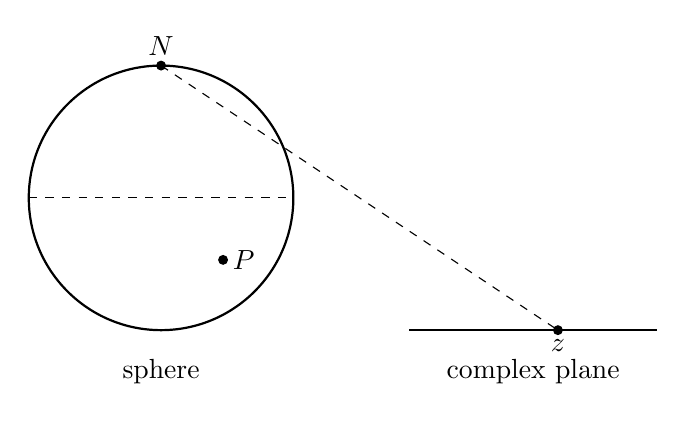
\begin{tikzpicture}[scale=1.05]
\draw[thick] (0,0) circle (1.6);
\draw[dashed] (-1.6,0)--(1.6,0);
\filldraw (0,1.6) circle (1.5pt) node[above] {$N$};
\filldraw (.75,-.75) circle (1.5pt) node[right] {$P$};

\draw[thick] (3,-1.6)--(6,-1.6);
\filldraw (4.8,-1.6) circle (1.5pt) node[below] {$z$};

\draw[dashed] (0,1.6)--(4.8,-1.6);

\node at (0,-2.1) {sphere};
\node at (4.5,-2.1) {complex plane};
\end{tikzpicture}
\end{centereddiagram}

The north pole corresponds to

\[
\infty.
\]

All other points correspond to finite complex numbers.

%%%%%%%%%%%%%%%%%%%%%%%%%%%%%%%%%%%%%%%%%%%%%%%%%%%%%%%%%%%%
\subsection{Complex Projective Space}
\label{subsec:complex-projective-space}
%%%%%%%%%%%%%%%%%%%%%%%%%%%%%%%%%%%%%%%%%%%%%%%%%%%%%%%%%%%%

Complex projective space is

\[
\boxed{
\mathbb{P}^n_{\C}
=
\left(
\C^{n+1}\setminus\{0\}
\right)/\sim
}
\]

where

\[
(z_0,\ldots,z_n)
\sim
(\lambda z_0,\ldots,\lambda z_n)
\]

for every

\[
\lambda\in\C^\times.
\]

A point is written

\[
\boxed{
[z_0:z_1:\cdots:z_n].
}
\]

The space

\[
\mathbb{P}^n_{\C}
\]

has complex dimension

\[
\boxed{n}
\]

and real dimension

\[
\boxed{2n.}
\]

%%%%%%%%%%%%%%%%%%%%%%%%%%%%%%%%%%%%%%%%%%%%%%%%%%%%%%%%%%%%
\subsection{Affine Charts on Complex Projective Space}
\label{subsec:complex-projective-affine-charts}
%%%%%%%%%%%%%%%%%%%%%%%%%%%%%%%%%%%%%%%%%%%%%%%%%%%%%%%%%%%%

For each \(j\), define

\[
U_j
=
\{
[z_0:\cdots:z_n]:
z_j\neq0
\}.
\]

On \(U_j\), divide every coordinate by \(z_j\).

For example, on

\[
U_0,
\]

we obtain coordinates

\[
\boxed{
\left(
\frac{z_1}{z_0},
\ldots,
\frac{z_n}{z_0}
\right)\in\C^n.
}
\]

Thus

\[
U_0\cong\C^n.
\]

The transition maps between these charts are holomorphic, making

\[
\mathbb{P}^n_{\C}
\]

a complex manifold.

%%%%%%%%%%%%%%%%%%%%%%%%%%%%%%%%%%%%%%%%%%%%%%%%%%%%%%%%%%%%
\subsection{Complex Tori}
\label{subsec:complex-tori}
%%%%%%%%%%%%%%%%%%%%%%%%%%%%%%%%%%%%%%%%%%%%%%%%%%%%%%%%%%%%

Let

\[
\Lambda
=
\Z\omega_1+\Z\omega_2
\subseteq\C
\]

be a lattice generated by two complex numbers that are linearly independent
over \(\R\).

\begin{definitionbox}{Complex Torus}
The quotient

\[
\boxed{
\C/\Lambda
}
\]

is a one-dimensional \emph{complex torus}.
\end{definitionbox}

Topologically,

\[
\C/\Lambda
\]

is a torus.

Complex analytically, it is a compact Riemann surface.

%%%%%%%%%%%%%%%%%%%%%%%%%%%%%%%%%%%%%%%%%%%%%%%%%%%%%%%%%%%%
\subsection{Complex Tori and Elliptic Curves}
\label{subsec:complex-tori-elliptic-curves}
%%%%%%%%%%%%%%%%%%%%%%%%%%%%%%%%%%%%%%%%%%%%%%%%%%%%%%%%%%%%

Every complex elliptic curve can be represented analytically as

\[
\boxed{
E\cong\C/\Lambda
}
\]

for a suitable lattice \(\Lambda\).

It can also be represented algebraically by a nonsingular cubic equation,
such as

\[
\boxed{
y^2=x^3+Ax+B.
}
\]

Thus the same object can be studied from several perspectives:

\[
\boxed{
\begin{array}{c}
\text{complex torus}\\
\Updownarrow\\
\text{compact genus-one Riemann surface}\\
\Updownarrow\\
\text{complex elliptic curve}
\end{array}
}
\]

This is a major example of the interaction between complex analysis and
algebraic geometry.

%%%%%%%%%%%%%%%%%%%%%%%%%%%%%%%%%%%%%%%%%%%%%%%%%%%%%%%%%%%%
\subsection{Almost Complex Structures}
\label{subsec:almost-complex-structures}
%%%%%%%%%%%%%%%%%%%%%%%%%%%%%%%%%%%%%%%%%%%%%%%%%%%%%%%%%%%%

Complex multiplication by \(i\) suggests an intrinsic description of complex
geometry.

\begin{definitionbox}{Almost Complex Structure}
An \emph{almost complex structure} on a smooth manifold \(M\) is a smooth
bundle map

\[
\boxed{
J:TM\to TM
}
\]

satisfying

\[
\boxed{
J^2=-I.
}
\]
\end{definitionbox}

Here \(I\) denotes the identity transformation.

The map \(J\) behaves like multiplication by

\[
i.
\]

%%%%%%%%%%%%%%%%%%%%%%%%%%%%%%%%%%%%%%%%%%%%%%%%%%%%%%%%%%%%
\subsection{Geometric Meaning of \(J\)}
\label{subsec:geometric-meaning-j}
%%%%%%%%%%%%%%%%%%%%%%%%%%%%%%%%%%%%%%%%%%%%%%%%%%%%%%%%%%%%

In the complex plane,

\[
z=x+iy.
\]

Multiplication by \(i\) gives

\[
iz=-y+ix.
\]

In real coordinates this corresponds to

\[
\boxed{
J
\begin{pmatrix}
x\\y
\end{pmatrix}
=
\begin{pmatrix}
-y\\x
\end{pmatrix}.
}
\]

Thus \(J\) acts as a \(90^\circ\) rotation on each complex coordinate plane.

Applying it twice gives

\[
J^2=-I.
\]

%%%%%%%%%%%%%%%%%%%%%%%%%%%%%%%%%%%%%%%%%%%%%%%%%%%%%%%%%%%%
\subsection{Complex Structures and Integrability}
\label{subsec:complex-integrability}
%%%%%%%%%%%%%%%%%%%%%%%%%%%%%%%%%%%%%%%%%%%%%%%%%%%%%%%%%%%%

Every complex manifold determines an almost complex structure.

However, not every almost complex structure comes from holomorphic
coordinates.

An almost complex structure that does arise from genuine complex coordinate
charts is called \emph{integrable}.

Thus

\[
\boxed{
\text{complex structure}
=
\text{integrable almost complex structure}.
}
\]

The obstruction to integrability is measured by the Nijenhuis tensor.

%%%%%%%%%%%%%%%%%%%%%%%%%%%%%%%%%%%%%%%%%%%%%%%%%%%%%%%%%%%%
\subsection{Newlander--Nirenberg Theorem}
\label{subsec:newlander-nirenberg}
%%%%%%%%%%%%%%%%%%%%%%%%%%%%%%%%%%%%%%%%%%%%%%%%%%%%%%%%%%%%

A fundamental result connects the differential-geometric and
complex-analytic descriptions.

\begin{theorem}[Newlander--Nirenberg]
An almost complex structure \(J\) is integrable if and only if its Nijenhuis
tensor vanishes.
\end{theorem}

Schematically,

\[
\boxed{
N_J=0
\quad\Longleftrightarrow\quad
\text{local holomorphic coordinates exist}.
}
\]

This theorem gives an intrinsic criterion for determining whether an almost
complex manifold is actually a complex manifold.

%%%%%%%%%%%%%%%%%%%%%%%%%%%%%%%%%%%%%%%%%%%%%%%%%%%%%%%%%%%%
\subsection{Complexified Tangent Spaces}
\label{subsec:complexified-tangent-spaces}
%%%%%%%%%%%%%%%%%%%%%%%%%%%%%%%%%%%%%%%%%%%%%%%%%%%%%%%%%%%%

Let \(M\) be a complex manifold.

Its real tangent bundle may be complexified:

\[
\boxed{
T_{\C}M
=
TM\otimes_{\R}\C.
}
\]

The almost complex structure \(J\) extends complex-linearly.

Since

\[
J^2=-I,
\]

its eigenvalues over \(\C\) are

\[
\boxed{i\quad\text{and}\quad -i.}
\]

This produces a fundamental decomposition.

%%%%%%%%%%%%%%%%%%%%%%%%%%%%%%%%%%%%%%%%%%%%%%%%%%%%%%%%%%%%
\subsection{Holomorphic and Antiholomorphic Tangent Directions}
\label{subsec:holomorphic-antiholomorphic-directions}
%%%%%%%%%%%%%%%%%%%%%%%%%%%%%%%%%%%%%%%%%%%%%%%%%%%%%%%%%%%%

The complexified tangent bundle decomposes as

\[
\boxed{
T_{\C}M
=
T^{1,0}M
\oplus
T^{0,1}M.
}
\]

The space

\[
T^{1,0}M
\]

is the \(i\)-eigenspace of \(J\), while

\[
T^{0,1}M
\]

is the \(-i\)-eigenspace.

These are called the holomorphic and antiholomorphic tangent bundles,
respectively.

%%%%%%%%%%%%%%%%%%%%%%%%%%%%%%%%%%%%%%%%%%%%%%%%%%%%%%%%%%%%
\subsection{Wirtinger Derivatives}
\label{subsec:wirtinger-derivatives}
%%%%%%%%%%%%%%%%%%%%%%%%%%%%%%%%%%%%%%%%%%%%%%%%%%%%%%%%%%%%

For

\[
z=x+iy,
\qquad
\bar z=x-iy,
\]

define

\[
\boxed{
\frac{\partial}{\partial z}
=
\frac12
\left(
\frac{\partial}{\partial x}
-
i\frac{\partial}{\partial y}
\right)
}
\]

and

\[
\boxed{
\frac{\partial}{\partial\bar z}
=
\frac12
\left(
\frac{\partial}{\partial x}
+
i\frac{\partial}{\partial y}
\right).
}
\]

These are called \emph{Wirtinger derivatives}.

%%%%%%%%%%%%%%%%%%%%%%%%%%%%%%%%%%%%%%%%%%%%%%%%%%%%%%%%%%%%
\subsection{Holomorphicity Using \(\bar{\partial}\)}
\label{subsec:holomorphicity-bar-partial}
%%%%%%%%%%%%%%%%%%%%%%%%%%%%%%%%%%%%%%%%%%%%%%%%%%%%%%%%%%%%

A sufficiently differentiable function

\[
f:\C\to\C
\]

is holomorphic precisely when

\[
\boxed{
\frac{\partial f}{\partial\bar z}=0.
}
\]

In several variables,

\[
f(z_1,\ldots,z_n)
\]

is holomorphic when

\[
\boxed{
\frac{\partial f}{\partial\bar z_j}=0
\qquad
\text{for every }j.
}
\]

This compactly expresses the Cauchy--Riemann equations.

%%%%%%%%%%%%%%%%%%%%%%%%%%%%%%%%%%%%%%%%%%%%%%%%%%%%%%%%%%%%
\subsection{Complex Differential Forms}
\label{subsec:complex-differential-forms}
%%%%%%%%%%%%%%%%%%%%%%%%%%%%%%%%%%%%%%%%%%%%%%%%%%%%%%%%%%%%

Since

\[
z=x+iy,
\]

we have

\[
\boxed{
dz=dx+i\,dy
}
\]

and

\[
\boxed{
d\bar z=dx-i\,dy.
}
\]

These forms provide natural bases for differential forms on complex
manifolds.

In several variables,

\[
dz_1,\ldots,dz_n
\]

represent holomorphic directions, while

\[
d\bar z_1,\ldots,d\bar z_n
\]

represent antiholomorphic directions.

%%%%%%%%%%%%%%%%%%%%%%%%%%%%%%%%%%%%%%%%%%%%%%%%%%%%%%%%%%%%
\subsection{Forms of Type \((p,q)\)}
\label{subsec:pq-forms}
%%%%%%%%%%%%%%%%%%%%%%%%%%%%%%%%%%%%%%%%%%%%%%%%%%%%%%%%%%%%

Complex differential forms decompose according to the number of holomorphic
and antiholomorphic factors.

\begin{definitionbox}{Form of Type \((p,q)\)}
A differential form is of \emph{type \((p,q)\)} if locally it is a sum of
terms containing \(p\) factors of the form \(dz_j\) and \(q\) factors of the
form \(d\bar z_k\).
\end{definitionbox}

A typical term is

\[
\boxed{
f\,
dz_{i_1}\wedge\cdots\wedge dz_{i_p}
\wedge
d\bar z_{j_1}\wedge\cdots\wedge d\bar z_{j_q}.
}
\]

%%%%%%%%%%%%%%%%%%%%%%%%%%%%%%%%%%%%%%%%%%%%%%%%%%%%%%%%%%%%
\subsection{Examples of Form Types}
\label{subsec:examples-form-types}
%%%%%%%%%%%%%%%%%%%%%%%%%%%%%%%%%%%%%%%%%%%%%%%%%%%%%%%%%%%%

The form

\[
dz_1
\]

has type

\[
\boxed{(1,0).}
\]

The form

\[
d\bar z_1
\]

has type

\[
\boxed{(0,1).}
\]

The form

\[
dz_1\wedge dz_2
\]

has type

\[
\boxed{(2,0).}
\]

The form

\[
dz_1\wedge d\bar z_2
\]

has type

\[
\boxed{(1,1).}
\]

%%%%%%%%%%%%%%%%%%%%%%%%%%%%%%%%%%%%%%%%%%%%%%%%%%%%%%%%%%%%
\subsection{Decomposition of Differential Forms}
\label{subsec:complex-form-decomposition}
%%%%%%%%%%%%%%%%%%%%%%%%%%%%%%%%%%%%%%%%%%%%%%%%%%%%%%%%%%%%

On a complex manifold,

\[
\boxed{
\Omega^k_{\C}(M)
=
\bigoplus_{p+q=k}
\Omega^{p,q}(M).
}
\]

Thus a complex-valued \(k\)-form can be decomposed according to its
\((p,q)\)-types.

For example,

\[
\Omega^2_{\C}(M)
=
\Omega^{2,0}(M)
\oplus
\Omega^{1,1}(M)
\oplus
\Omega^{0,2}(M).
\]

%%%%%%%%%%%%%%%%%%%%%%%%%%%%%%%%%%%%%%%%%%%%%%%%%%%%%%%%%%%%
\subsection{The Operators \(\partial\) and \(\bar{\partial}\)}
\label{subsec:partial-barpartial}
%%%%%%%%%%%%%%%%%%%%%%%%%%%%%%%%%%%%%%%%%%%%%%%%%%%%%%%%%%%%

On a complex manifold, the exterior derivative decomposes as

\[
\boxed{
d=\partial+\bar{\partial}.
}
\]

The operator

\[
\partial
\]

raises the holomorphic degree:

\[
\boxed{
\partial:
\Omega^{p,q}
\to
\Omega^{p+1,q}.
}
\]

The operator

\[
\bar{\partial}
\]

raises the antiholomorphic degree:

\[
\boxed{
\bar{\partial}:
\Omega^{p,q}
\to
\Omega^{p,q+1}.
}
\]

%%%%%%%%%%%%%%%%%%%%%%%%%%%%%%%%%%%%%%%%%%%%%%%%%%%%%%%%%%%%
\subsection{Relations Among the Differential Operators}
\label{subsec:complex-differential-relations}
%%%%%%%%%%%%%%%%%%%%%%%%%%%%%%%%%%%%%%%%%%%%%%%%%%%%%%%%%%%%

Since

\[
d^2=0,
\]

the decomposition

\[
d=\partial+\bar{\partial}
\]

implies

\[
\boxed{\partial^2=0,}
\]

\[
\boxed{\bar{\partial}^2=0,}
\]

and

\[
\boxed{
\partial\bar{\partial}
+
\bar{\partial}\partial
=
0.
}
\]

These identities form the basis of Dolbeault theory.

%%%%%%%%%%%%%%%%%%%%%%%%%%%%%%%%%%%%%%%%%%%%%%%%%%%%%%%%%%%%
\subsection{Dolbeault Cohomology}
\label{subsec:dolbeault-cohomology}
%%%%%%%%%%%%%%%%%%%%%%%%%%%%%%%%%%%%%%%%%%%%%%%%%%%%%%%%%%%%

Because

\[
\bar{\partial}^2=0,
\]

one obtains a cohomology theory.

\begin{definitionbox}{Dolbeault Cohomology}
The \emph{Dolbeault cohomology groups} are

\[
\boxed{
H_{\bar{\partial}}^{p,q}(M)
=
\frac{
\ker\left(
\bar{\partial}:\Omega^{p,q}\to\Omega^{p,q+1}
\right)
}{
\operatorname{im}\left(
\bar{\partial}:\Omega^{p,q-1}\to\Omega^{p,q}
\right)
}.
}
\]
\end{definitionbox}

Dolbeault cohomology measures global properties of complex manifolds that
cannot generally be detected from local coordinates alone.

%%%%%%%%%%%%%%%%%%%%%%%%%%%%%%%%%%%%%%%%%%%%%%%%%%%%%%%%%%%%
\subsection{Hermitian Metrics}
\label{subsec:hermitian-metrics}
%%%%%%%%%%%%%%%%%%%%%%%%%%%%%%%%%%%%%%%%%%%%%%%%%%%%%%%%%%%%

A Riemannian metric measures lengths and angles on a real manifold.

A complex manifold has an analogous structure compatible with complex
multiplication.

\begin{definitionbox}{Hermitian Metric}
A \emph{Hermitian metric} on a complex manifold is a smoothly varying
positive-definite Hermitian inner product on its complex tangent spaces.
\end{definitionbox}

Locally it can be written

\[
\boxed{
h
=
\sum_{j,k}
h_{j\bar k}\,
dz_j\otimes d\bar z_k.
}
\]

%%%%%%%%%%%%%%%%%%%%%%%%%%%%%%%%%%%%%%%%%%%%%%%%%%%%%%%%%%%%
\subsection{Hermitian Symmetry}
\label{subsec:hermitian-symmetry}
%%%%%%%%%%%%%%%%%%%%%%%%%%%%%%%%%%%%%%%%%%%%%%%%%%%%%%%%%%%%

A Hermitian inner product satisfies

\[
\boxed{
h(u,v)
=
\overline{h(v,u)}.
}
\]

It is complex-linear in one argument and conjugate-linear in the other,
depending on the convention being used.

Positive definiteness means

\[
\boxed{
h(v,v)>0
}
\]

for every nonzero tangent vector \(v\).

%%%%%%%%%%%%%%%%%%%%%%%%%%%%%%%%%%%%%%%%%%%%%%%%%%%%%%%%%%%%
\subsection{Compatible Riemannian Metrics}
\label{subsec:compatible-riemannian-metric}
%%%%%%%%%%%%%%%%%%%%%%%%%%%%%%%%%%%%%%%%%%%%%%%%%%%%%%%%%%%%

An almost complex structure \(J\) and Riemannian metric \(g\) are compatible
when

\[
\boxed{
g(JX,JY)=g(X,Y).
}
\]

Thus multiplication by \(i\) preserves lengths and angles.

A compatible pair

\[
(g,J)
\]

determines a Hermitian structure.

%%%%%%%%%%%%%%%%%%%%%%%%%%%%%%%%%%%%%%%%%%%%%%%%%%%%%%%%%%%%
\subsection{The Fundamental Two-Form}
\label{subsec:fundamental-two-form}
%%%%%%%%%%%%%%%%%%%%%%%%%%%%%%%%%%%%%%%%%%%%%%%%%%%%%%%%%%%%

Given a compatible metric \(g\) and complex structure \(J\), define

\[
\boxed{
\omega(X,Y)=g(JX,Y).
}
\]

The lowercase Greek letter

\[
\omega
\]

is read ``omega.''

The form \(\omega\) is called the \emph{fundamental form}, or in the
K\"ahler setting, the \emph{K\"ahler form}.

It is a real differential \(2\)-form of type

\[
(1,1).
\]

%%%%%%%%%%%%%%%%%%%%%%%%%%%%%%%%%%%%%%%%%%%%%%%%%%%%%%%%%%%%
\subsection{K\"ahler Manifolds}
\label{subsec:kahler-manifolds}
%%%%%%%%%%%%%%%%%%%%%%%%%%%%%%%%%%%%%%%%%%%%%%%%%%%%%%%%%%%%

One of the most important structures in complex geometry combines complex,
Riemannian, and symplectic geometry.

\begin{definitionbox}{K\"ahler Manifold}
A \emph{K\"ahler manifold} is a complex manifold equipped with a Hermitian
metric whose fundamental \(2\)-form \(\omega\) satisfies

\[
\boxed{d\omega=0.}
\]
\end{definitionbox}

Thus a K\"ahler manifold simultaneously carries compatible

\[
\boxed{
\text{complex},
\qquad
\text{Riemannian},
\qquad
\text{symplectic}
}
\]

structures.

%%%%%%%%%%%%%%%%%%%%%%%%%%%%%%%%%%%%%%%%%%%%%%%%%%%%%%%%%%%%
\subsection{The K\"ahler Triangle}
\label{subsec:kahler-triangle}
%%%%%%%%%%%%%%%%%%%%%%%%%%%%%%%%%%%%%%%%%%%%%%%%%%%%%%%%%%%%

The K\"ahler condition creates a remarkable intersection of three geometric
theories.

\begin{centereddiagram}
\begin{tikzpicture}[
every node/.style={align=center}
]
\node[draw,rounded corners,minimum width=3cm,minimum height=8mm]
(C) at (0,2.5) {Complex\\Geometry};

\node[draw,rounded corners,minimum width=3cm,minimum height=8mm]
(R) at (-3,-1) {Riemannian\\Geometry};

\node[draw,rounded corners,minimum width=3cm,minimum height=8mm]
(S) at (3,-1) {Symplectic\\Geometry};

\node[draw,rounded corners,fill=gray!8]
(K) at (0,.2) {K\"ahler\\Geometry};

\draw[-{Latex[length=3mm]}] (K)--(C);
\draw[-{Latex[length=3mm]}] (K)--(R);
\draw[-{Latex[length=3mm]}] (K)--(S);
\end{tikzpicture}
\end{centereddiagram}

This interaction is one reason K\"ahler geometry is so powerful.

%%%%%%%%%%%%%%%%%%%%%%%%%%%%%%%%%%%%%%%%%%%%%%%%%%%%%%%%%%%%
\subsection{Examples of K\"ahler Manifolds}
\label{subsec:kahler-examples}
%%%%%%%%%%%%%%%%%%%%%%%%%%%%%%%%%%%%%%%%%%%%%%%%%%%%%%%%%%%%

Important examples include:

\[
\boxed{\C^n,}
\]

complex projective space

\[
\boxed{\mathbb{P}^n_{\C},}
\]

complex tori,

\[
\boxed{\C^n/\Lambda,}
\]

and smooth complex projective varieties.

Every Riemann surface admits a K\"ahler structure.

%%%%%%%%%%%%%%%%%%%%%%%%%%%%%%%%%%%%%%%%%%%%%%%%%%%%%%%%%%%%
\subsection{The Standard K\"ahler Form on \(\C^n\)}
\label{subsec:standard-kahler-form}
%%%%%%%%%%%%%%%%%%%%%%%%%%%%%%%%%%%%%%%%%%%%%%%%%%%%%%%%%%%%

For

\[
z_j=x_j+iy_j,
\]

the standard K\"ahler form on \(\C^n\) is

\[
\boxed{
\omega
=
\sum_{j=1}^{n}
dx_j\wedge dy_j.
}
\]

Equivalently,

\[
\boxed{
\omega
=
\frac{i}{2}
\sum_{j=1}^{n}
dz_j\wedge d\bar z_j.
}
\]

Since the coefficients are constant,

\[
d\omega=0.
\]

Therefore \(\C^n\) is K\"ahler.

%%%%%%%%%%%%%%%%%%%%%%%%%%%%%%%%%%%%%%%%%%%%%%%%%%%%%%%%%%%%
\subsection{K\"ahler Potentials}
\label{subsec:kahler-potentials}
%%%%%%%%%%%%%%%%%%%%%%%%%%%%%%%%%%%%%%%%%%%%%%%%%%%%%%%%%%%%

Locally, a K\"ahler form can often be expressed using a real-valued function

\[
\varphi.
\]

The lowercase Greek letter

\[
\varphi
\]

is read ``phi.''

Locally,

\[
\boxed{
\omega
=
i\partial\bar{\partial}\varphi.
}
\]

The function \(\varphi\) is called a \emph{K\"ahler potential}.

For flat \(\C^n\), one may use

\[
\boxed{
\varphi(z)
=
\frac12
\sum_{j=1}^{n}|z_j|^2.
}
\]

%%%%%%%%%%%%%%%%%%%%%%%%%%%%%%%%%%%%%%%%%%%%%%%%%%%%%%%%%%%%
\subsection{The Fubini--Study Metric}
\label{subsec:fubini-study}
%%%%%%%%%%%%%%%%%%%%%%%%%%%%%%%%%%%%%%%%%%%%%%%%%%%%%%%%%%%%

Complex projective space carries a canonical K\"ahler metric called the
\emph{Fubini--Study metric}.

On an affine chart with coordinates

\[
z=(z_1,\ldots,z_n),
\]

a K\"ahler potential is

\[
\boxed{
\varphi(z)
=
\log
\left(
1+\sum_{j=1}^{n}|z_j|^2
\right).
}
\]

The associated K\"ahler form is

\[
\boxed{
\omega_{\mathrm{FS}}
=
i\partial\bar{\partial}
\log
\left(
1+\sum_{j=1}^{n}|z_j|^2
\right).
}
\]

This metric is central in complex and algebraic geometry.

%%%%%%%%%%%%%%%%%%%%%%%%%%%%%%%%%%%%%%%%%%%%%%%%%%%%%%%%%%%%
\subsection{Holomorphic Differential Forms}
\label{subsec:holomorphic-differential-forms}
%%%%%%%%%%%%%%%%%%%%%%%%%%%%%%%%%%%%%%%%%%%%%%%%%%%%%%%%%%%%

A \((p,0)\)-form

\[
\alpha
\]

is holomorphic when its local coefficient functions are holomorphic.

For example, on \(\C^n\),

\[
\boxed{
dz_1\wedge\cdots\wedge dz_n
}
\]

is a holomorphic \(n\)-form.

Holomorphic differential forms carry important information about the global
geometry of a complex manifold.

%%%%%%%%%%%%%%%%%%%%%%%%%%%%%%%%%%%%%%%%%%%%%%%%%%%%%%%%%%%%
\subsection{The Canonical Bundle}
\label{subsec:canonical-bundle-complex}
%%%%%%%%%%%%%%%%%%%%%%%%%%%%%%%%%%%%%%%%%%%%%%%%%%%%%%%%%%%%

On a complex \(n\)-manifold, the bundle of holomorphic \(n\)-forms is called
the \emph{canonical bundle}.

It is denoted

\[
\boxed{
K_M
=
\Lambda^n(T^{1,0}M)^*.
}
\]

Sections of \(K_M\) are holomorphic top-degree forms.

The canonical bundle is one of the most important line bundles in complex
and algebraic geometry.

%%%%%%%%%%%%%%%%%%%%%%%%%%%%%%%%%%%%%%%%%%%%%%%%%%%%%%%%%%%%
\subsection{Canonical Bundle Examples}
\label{subsec:canonical-bundle-examples}
%%%%%%%%%%%%%%%%%%%%%%%%%%%%%%%%%%%%%%%%%%%%%%%%%%%%%%%%%%%%

On \(\C^n\),

\[
dz_1\wedge\cdots\wedge dz_n
\]

is a nowhere-vanishing holomorphic section of the canonical bundle.

Therefore

\[
\boxed{
K_{\C^n}
\text{ is trivial}.
}
\]

For complex projective space,

\[
\boxed{
K_{\mathbb{P}^n}
\cong
\mathcal{O}(-n-1).
}
\]

The behavior of the canonical bundle plays a major role in the classification
of complex manifolds and algebraic varieties.

%%%%%%%%%%%%%%%%%%%%%%%%%%%%%%%%%%%%%%%%%%%%%%%%%%%%%%%%%%%%
\subsection{Holomorphic Vector Bundles}
\label{subsec:holomorphic-vector-bundles}
%%%%%%%%%%%%%%%%%%%%%%%%%%%%%%%%%%%%%%%%%%%%%%%%%%%%%%%%%%%%

A holomorphic vector bundle is a complex vector bundle whose transition
functions are holomorphic.

Locally,

\[
E|_U\cong U\times\C^r.
\]

Examples include:

\begin{itemize}
    \item the holomorphic tangent bundle \(T^{1,0}M\);
    \item the holomorphic cotangent bundle;
    \item the canonical bundle \(K_M\);
    \item holomorphic line bundles.
\end{itemize}

These bundles connect complex geometry with algebraic geometry and topology.

%%%%%%%%%%%%%%%%%%%%%%%%%%%%%%%%%%%%%%%%%%%%%%%%%%%%%%%%%%%%
\subsection{Divisors and Line Bundles}
\label{subsec:complex-divisors-line-bundles}
%%%%%%%%%%%%%%%%%%%%%%%%%%%%%%%%%%%%%%%%%%%%%%%%%%%%%%%%%%%%

On complex manifolds, zeros and poles of meromorphic functions naturally
produce divisors.

A divisor may be written schematically as

\[
\boxed{
D=\sum_j n_jD_j,
}
\]

where the \(D_j\) are irreducible codimension-one analytic subsets.

Under suitable conditions, divisors correspond to holomorphic line bundles.

This parallels the divisor theory developed in
\cref{sec:algebraic-geometry}.

%%%%%%%%%%%%%%%%%%%%%%%%%%%%%%%%%%%%%%%%%%%%%%%%%%%%%%%%%%%%
\subsection{Meromorphic Functions}
\label{subsec:complex-meromorphic-functions}
%%%%%%%%%%%%%%%%%%%%%%%%%%%%%%%%%%%%%%%%%%%%%%%%%%%%%%%%%%%%

A meromorphic function is locally a quotient

\[
\boxed{
f=\frac{g}{h}
}
\]

of holomorphic functions, where \(h\) is not identically zero.

Meromorphic functions may have poles.

On a compact Riemann surface, meromorphic functions play a role analogous to
rational functions on algebraic curves.

%%%%%%%%%%%%%%%%%%%%%%%%%%%%%%%%%%%%%%%%%%%%%%%%%%%%%%%%%%%%
\subsection{Compact Complex Manifolds}
\label{subsec:compact-complex-manifolds}
%%%%%%%%%%%%%%%%%%%%%%%%%%%%%%%%%%%%%%%%%%%%%%%%%%%%%%%%%%%%

Compactness imposes strong restrictions on holomorphic functions.

For example, if \(M\) is a connected compact complex manifold, every
holomorphic function

\[
f:M\to\C
\]

is constant.

This follows from the maximum modulus principle.

Thus global holomorphic function theory on compact complex manifolds can be
much more rigid than on noncompact spaces.

%%%%%%%%%%%%%%%%%%%%%%%%%%%%%%%%%%%%%%%%%%%%%%%%%%%%%%%%%%%%
\subsection{Complex Curves and Topology}
\label{subsec:complex-curves-topology}
%%%%%%%%%%%%%%%%%%%%%%%%%%%%%%%%%%%%%%%%%%%%%%%%%%%%%%%%%%%%

A compact connected Riemann surface is topologically an orientable surface.

Its topology is classified by its genus

\[
g.
\]

Examples include

\[
\boxed{
g=0:
\text{ sphere},
}
\]

\[
\boxed{
g=1:
\text{ torus},
}
\]

and

\[
\boxed{
g\geq2:
\text{ higher-genus surfaces}.
}
\]

The genus simultaneously appears in topology, algebraic geometry, and
complex analysis.

%%%%%%%%%%%%%%%%%%%%%%%%%%%%%%%%%%%%%%%%%%%%%%%%%%%%%%%%%%%%
\subsection{Uniformization of Riemann Surfaces}
\label{subsec:uniformization-riemann-surfaces}
%%%%%%%%%%%%%%%%%%%%%%%%%%%%%%%%%%%%%%%%%%%%%%%%%%%%%%%%%%%%

One of the central theorems of one-dimensional complex geometry is the
Uniformization Theorem.

\begin{theorem}[Uniformization Theorem]
Every simply connected Riemann surface is biholomorphic to exactly one of the
three standard types

\[
\boxed{
\mathbb{P}^1_{\C},
\qquad
\C,
\qquad
\mathbb{D},
}
\]

where

\[
\mathbb{D}
=
\{z\in\C:|z|<1\}
\]

is the unit disk.
\end{theorem}

Thus Riemann surfaces naturally divide into spherical, Euclidean, and
hyperbolic types.

%%%%%%%%%%%%%%%%%%%%%%%%%%%%%%%%%%%%%%%%%%%%%%%%%%%%%%%%%%%%
\subsection{Biholomorphic Maps}
\label{subsec:biholomorphic-maps}
%%%%%%%%%%%%%%%%%%%%%%%%%%%%%%%%%%%%%%%%%%%%%%%%%%%%%%%%%%%%

\begin{definitionbox}{Biholomorphism}
A map

\[
F:M\to N
\]

between complex manifolds is a \emph{biholomorphism} if \(F\) is holomorphic,
bijective, and its inverse

\[
F^{-1}:N\to M
\]

is also holomorphic.
\end{definitionbox}

Two biholomorphic complex manifolds are regarded as equivalent from the
complex-analytic viewpoint.

%%%%%%%%%%%%%%%%%%%%%%%%%%%%%%%%%%%%%%%%%%%%%%%%%%%%%%%%%%%%
\subsection{Holomorphic Versus Smooth Equivalence}
\label{subsec:holomorphic-vs-smooth}
%%%%%%%%%%%%%%%%%%%%%%%%%%%%%%%%%%%%%%%%%%%%%%%%%%%%%%%%%%%%

Two manifolds can be diffeomorphic as smooth manifolds while possessing
different complex structures.

Thus

\[
\boxed{
\text{same smooth manifold}
\not\Longrightarrow
\text{same complex manifold}.
}
\]

Complex geometry therefore contains finer information than ordinary smooth
geometry.

%%%%%%%%%%%%%%%%%%%%%%%%%%%%%%%%%%%%%%%%%%%%%%%%%%%%%%%%%%%%
\subsection{Hodge Theory}
\label{subsec:hodge-theory-complex}
%%%%%%%%%%%%%%%%%%%%%%%%%%%%%%%%%%%%%%%%%%%%%%%%%%%%%%%%%%%%

Hodge theory connects topology, differential geometry, and complex geometry.

On a compact K\"ahler manifold, complex cohomology decomposes according to
\((p,q)\)-type:

\[
\boxed{
H^k(M,\C)
\cong
\bigoplus_{p+q=k}
H^{p,q}(M).
}
\]

The dimensions

\[
\boxed{
h^{p,q}
=
\dim_{\C}H^{p,q}(M)
}
\]

are called \emph{Hodge numbers}.

%%%%%%%%%%%%%%%%%%%%%%%%%%%%%%%%%%%%%%%%%%%%%%%%%%%%%%%%%%%%
\subsection{The Hodge Diamond}
\label{subsec:hodge-diamond}
%%%%%%%%%%%%%%%%%%%%%%%%%%%%%%%%%%%%%%%%%%%%%%%%%%%%%%%%%%%%

Hodge numbers are often arranged in a diamond.

For a complex surface, the pattern is

\[
\boxed{
\begin{array}{ccccc}
&&h^{0,0}&&\\
&h^{1,0}&&h^{0,1}&\\
h^{2,0}&&h^{1,1}&&h^{0,2}\\
&h^{2,1}&&h^{1,2}&\\
&&h^{2,2}&&
\end{array}
}
\]

Symmetries among these numbers reflect deep geometric structures.

For compact K\"ahler manifolds,

\[
\boxed{
h^{p,q}=h^{q,p}.
}
\]

%%%%%%%%%%%%%%%%%%%%%%%%%%%%%%%%%%%%%%%%%%%%%%%%%%%%%%%%%%%%
\subsection{Example: Hodge Diamond of \(\mathbb{P}^1\)}
\label{subsec:hodge-diamond-p1}
%%%%%%%%%%%%%%%%%%%%%%%%%%%%%%%%%%%%%%%%%%%%%%%%%%%%%%%%%%%%

For the complex projective line,

\[
\mathbb{P}^1_{\C},
\]

the nonzero Hodge numbers are

\[
h^{0,0}=1
\]

and

\[
h^{1,1}=1.
\]

Thus its Hodge diamond is

\[
\boxed{
\begin{array}{ccc}
&1&\\
0&&0\\
&1&
\end{array}
}
\]

which reflects the topology of the sphere.

%%%%%%%%%%%%%%%%%%%%%%%%%%%%%%%%%%%%%%%%%%%%%%%%%%%%%%%%%%%%
\subsection{Chern Classes}
\label{subsec:chern-classes-complex}
%%%%%%%%%%%%%%%%%%%%%%%%%%%%%%%%%%%%%%%%%%%%%%%%%%%%%%%%%%%%

Complex vector bundles possess characteristic classes called
\emph{Chern classes}.

For a complex vector bundle \(E\),

\[
\boxed{
c_k(E)\in H^{2k}(M,\Z).
}
\]

The total Chern class is

\[
\boxed{
c(E)
=
1+c_1(E)+c_2(E)+\cdots.
}
\]

Chern classes measure topological twisting of complex vector bundles and are
fundamental in complex and algebraic geometry.

%%%%%%%%%%%%%%%%%%%%%%%%%%%%%%%%%%%%%%%%%%%%%%%%%%%%%%%%%%%%
\subsection{First Chern Class}
\label{subsec:first-chern-class}
%%%%%%%%%%%%%%%%%%%%%%%%%%%%%%%%%%%%%%%%%%%%%%%%%%%%%%%%%%%%

For a complex line bundle \(L\), the primary characteristic class is

\[
\boxed{
c_1(L)\in H^2(M,\Z).
}
\]

The first Chern class connects:

\begin{itemize}
    \item topology;
    \item curvature;
    \item divisors;
    \item holomorphic line bundles;
    \item algebraic geometry.
\end{itemize}

For the canonical bundle \(K_M\),

\[
c_1(K_M)
\]

is closely related to the curvature and classification of \(M\).

%%%%%%%%%%%%%%%%%%%%%%%%%%%%%%%%%%%%%%%%%%%%%%%%%%%%%%%%%%%%
\subsection{Curvature in Complex Geometry}
\label{subsec:curvature-complex-geometry}
%%%%%%%%%%%%%%%%%%%%%%%%%%%%%%%%%%%%%%%%%%%%%%%%%%%%%%%%%%%%

Hermitian and K\"ahler metrics allow curvature to be studied using complex
coordinates.

Important curvature quantities include:

\begin{itemize}
    \item holomorphic sectional curvature;
    \item Ricci curvature;
    \item scalar curvature;
    \item curvature of holomorphic vector bundles.
\end{itemize}

In K\"ahler geometry, the compatibility of the complex and metric structures
greatly simplifies many curvature calculations.

%%%%%%%%%%%%%%%%%%%%%%%%%%%%%%%%%%%%%%%%%%%%%%%%%%%%%%%%%%%%
\subsection{The Ricci Form}
\label{subsec:ricci-form-complex}
%%%%%%%%%%%%%%%%%%%%%%%%%%%%%%%%%%%%%%%%%%%%%%%%%%%%%%%%%%%%

For a K\"ahler metric with local matrix

\[
(g_{j\bar k}),
\]

the Ricci form can be expressed locally as

\[
\boxed{
\rho
=
-i\partial\bar{\partial}
\log\det(g_{j\bar k}).
}
\]

The lowercase Greek letter

\[
\rho
\]

is read ``rho.''

The Ricci form represents, up to normalization conventions, the first Chern
class of the tangent bundle.

%%%%%%%%%%%%%%%%%%%%%%%%%%%%%%%%%%%%%%%%%%%%%%%%%%%%%%%%%%%%
\subsection{K\"ahler--Einstein Metrics}
\label{subsec:kahler-einstein}
%%%%%%%%%%%%%%%%%%%%%%%%%%%%%%%%%%%%%%%%%%%%%%%%%%%%%%%%%%%%

A K\"ahler metric is called \emph{K\"ahler--Einstein} when its Ricci form is
proportional to its K\"ahler form:

\[
\boxed{
\rho=\lambda\omega.
}
\]

The lowercase Greek letter

\[
\lambda
\]

is read ``lambda.''

The sign of \(\lambda\) is closely related to the geometry of the canonical
bundle and the first Chern class.

%%%%%%%%%%%%%%%%%%%%%%%%%%%%%%%%%%%%%%%%%%%%%%%%%%%%%%%%%%%%
\subsection{Calabi--Yau Manifolds}
\label{subsec:calabi-yau-manifolds}
%%%%%%%%%%%%%%%%%%%%%%%%%%%%%%%%%%%%%%%%%%%%%%%%%%%%%%%%%%%%

One important class of complex manifolds arises when the canonical bundle
has special behavior.

A commonly used geometric description of a Calabi--Yau manifold involves a
compact K\"ahler manifold with trivial canonical bundle, together with
additional hypotheses depending on convention.

Schematically,

\[
\boxed{
K_M\cong\mathcal{O}_M.
}
\]

Such a manifold admits a nowhere-vanishing holomorphic top form.

%%%%%%%%%%%%%%%%%%%%%%%%%%%%%%%%%%%%%%%%%%%%%%%%%%%%%%%%%%%%
\subsection{Calabi Conjecture and Yau's Theorem}
\label{subsec:calabi-yau-theorem}
%%%%%%%%%%%%%%%%%%%%%%%%%%%%%%%%%%%%%%%%%%%%%%%%%%%%%%%%%%%%

The Calabi conjecture asked whether a prescribed representative of the first
Chern class could be realized as the Ricci form of a K\"ahler metric.

Yau proved the conjecture.

One important consequence is that a compact K\"ahler manifold with vanishing
first Chern class admits a Ricci-flat K\"ahler metric in each K\"ahler class.

Thus

\[
\boxed{
c_1(M)=0
\quad\Longrightarrow\quad
\text{Ricci-flat K\"ahler geometry}
}
\]

under the hypotheses of the theorem.

%%%%%%%%%%%%%%%%%%%%%%%%%%%%%%%%%%%%%%%%%%%%%%%%%%%%%%%%%%%%
\subsection{Complex Submanifolds}
\label{subsec:complex-submanifolds}
%%%%%%%%%%%%%%%%%%%%%%%%%%%%%%%%%%%%%%%%%%%%%%%%%%%%%%%%%%%%

A complex submanifold is a subset that locally looks like a complex linear
subspace.

For example,

\[
\boxed{
\{(z_1,z_2)\in\C^2:z_2=0\}
}
\]

is a complex one-dimensional submanifold of \(\C^2\).

Its real dimension is

\[
2,
\]

while the ambient space has real dimension

\[
4.
\]

%%%%%%%%%%%%%%%%%%%%%%%%%%%%%%%%%%%%%%%%%%%%%%%%%%%%%%%%%%%%
\subsection{Holomorphic Implicit Function Theorem}
\label{subsec:holomorphic-implicit-function}
%%%%%%%%%%%%%%%%%%%%%%%%%%%%%%%%%%%%%%%%%%%%%%%%%%%%%%%%%%%%

Suppose

\[
F:\C^n\to\C^m
\]

is holomorphic.

If the complex Jacobian has maximal rank at a point, then locally the level
set

\[
F^{-1}(0)
\]

can be described as a complex submanifold.

Thus nonsingular polynomial equations over \(\C\) naturally produce complex
manifolds.

This provides a direct bridge from Algebraic Geometry to Complex Geometry.

%%%%%%%%%%%%%%%%%%%%%%%%%%%%%%%%%%%%%%%%%%%%%%%%%%%%%%%%%%%%
\subsection{Complex Algebraic Varieties}
\label{subsec:complex-algebraic-varieties}
%%%%%%%%%%%%%%%%%%%%%%%%%%%%%%%%%%%%%%%%%%%%%%%%%%%%%%%%%%%%

Suppose

\[
X\subseteq\C^n
\]

is defined by polynomial equations.

At a nonsingular point, \(X\) locally behaves like a complex manifold.

Therefore a smooth complex algebraic variety possesses both

\[
\boxed{
\text{algebraic structure}
}
\]

and

\[
\boxed{
\text{complex-analytic structure}.
}
\]

These structures interact in remarkably strong ways.

%%%%%%%%%%%%%%%%%%%%%%%%%%%%%%%%%%%%%%%%%%%%%%%%%%%%%%%%%%%%
\subsection{Analytification}
\label{subsec:analytification}
%%%%%%%%%%%%%%%%%%%%%%%%%%%%%%%%%%%%%%%%%%%%%%%%%%%%%%%%%%%%

A complex algebraic variety can be regarded as a complex analytic space.

This process is called \emph{analytification}.

Schematically,

\[
\boxed{
X
\longmapsto
X^{\mathrm{an}}.
}
\]

The notation

\[
X^{\mathrm{an}}
\]

is read ``X analytification'' or ``X analytic.''

Analytification allows analytic and topological tools to be applied to
algebraic varieties.

%%%%%%%%%%%%%%%%%%%%%%%%%%%%%%%%%%%%%%%%%%%%%%%%%%%%%%%%%%%%
\subsection{GAGA Philosophy}
\label{subsec:gaga-philosophy}
%%%%%%%%%%%%%%%%%%%%%%%%%%%%%%%%%%%%%%%%%%%%%%%%%%%%%%%%%%%%

For complex projective varieties, algebraic and analytic geometry are
especially closely related.

Serre's GAGA principles establish powerful correspondences between
algebraic and analytic objects in the projective setting.

Very schematically,

\[
\boxed{
\text{projective algebraic geometry over }\C
\quad\longleftrightarrow\quad
\text{compact complex analytic geometry}.
}
\]

This includes correspondences involving coherent sheaves and morphisms.

%%%%%%%%%%%%%%%%%%%%%%%%%%%%%%%%%%%%%%%%%%%%%%%%%%%%%%%%%%%%
\subsection{Stein Manifolds}
\label{subsec:stein-manifolds}
%%%%%%%%%%%%%%%%%%%%%%%%%%%%%%%%%%%%%%%%%%%%%%%%%%%%%%%%%%%%

Stein manifolds are complex manifolds that behave, in several important
ways, like affine algebraic varieties.

Examples include

\[
\boxed{\C^n}
\]

and many complex domains.

Stein manifolds possess abundant holomorphic functions and satisfy strong
cohomological vanishing properties.

They form a major class of noncompact complex manifolds.

%%%%%%%%%%%%%%%%%%%%%%%%%%%%%%%%%%%%%%%%%%%%%%%%%%%%%%%%%%%%
\subsection{Compact Versus Stein Geometry}
\label{subsec:compact-versus-stein}
%%%%%%%%%%%%%%%%%%%%%%%%%%%%%%%%%%%%%%%%%%%%%%%%%%%%%%%%%%%%

A useful broad contrast is

\[
\boxed{
\begin{array}{c|c}
\textbf{Compact Complex Geometry}
&
\textbf{Stein Geometry}
\\
\hline
\text{few global holomorphic functions}
&
\text{many holomorphic functions}
\\
\text{projective varieties often appear}
&
\text{affine-like behavior}
\\
\text{global topology prominent}
&
\text{function theory prominent}
\end{array}
}
\]

This contrast resembles the distinction between projective and affine
algebraic geometry.

%%%%%%%%%%%%%%%%%%%%%%%%%%%%%%%%%%%%%%%%%%%%%%%%%%%%%%%%%%%%
\subsection{Complex Geometry and Symplectic Geometry}
\label{subsec:complex-symplectic-connection}
%%%%%%%%%%%%%%%%%%%%%%%%%%%%%%%%%%%%%%%%%%%%%%%%%%%%%%%%%%%%

A K\"ahler manifold carries a closed nondegenerate \(2\)-form

\[
\omega.
\]

Therefore every K\"ahler manifold is naturally a symplectic manifold.

Hence

\[
\boxed{
\text{K\"ahler geometry}
\subseteq
\text{symplectic geometry}.
}
\]

However, not every symplectic manifold admits a compatible integrable complex
structure.

Symplectic Geometry is developed in
\cref{sec:symplectic-geometry}.

%%%%%%%%%%%%%%%%%%%%%%%%%%%%%%%%%%%%%%%%%%%%%%%%%%%%%%%%%%%%
\subsection{Complex Geometry and Algebraic Geometry}
\label{subsec:complex-algebraic-connection}
%%%%%%%%%%%%%%%%%%%%%%%%%%%%%%%%%%%%%%%%%%%%%%%%%%%%%%%%%%%%

Smooth projective varieties over \(\C\) are simultaneously

\begin{itemize}
    \item algebraic varieties;
    \item complex manifolds;
    \item smooth real manifolds;
    \item K\"ahler manifolds.
\end{itemize}

This creates a chain of perspectives:

\[
\boxed{
\text{polynomial equations}
\longrightarrow
\text{complex manifolds}
\longrightarrow
\text{smooth topology}.
}
\]

Information can often be transferred among these viewpoints.

%%%%%%%%%%%%%%%%%%%%%%%%%%%%%%%%%%%%%%%%%%%%%%%%%%%%%%%%%%%%
\subsection{Complex Geometry and Topology}
\label{subsec:complex-geometry-topology}
%%%%%%%%%%%%%%%%%%%%%%%%%%%%%%%%%%%%%%%%%%%%%%%%%%%%%%%%%%%%

Complex structures strongly constrain topology.

For example, every complex manifold is naturally orientable.

Compact K\"ahler manifolds satisfy additional restrictions arising from
Hodge theory.

Topological invariants used in complex geometry include

\[
\boxed{
\pi_1(M),
\quad
H^k(M),
\quad
c_k(M),
\quad
\chi(M).
}
\]

Here

\[
\chi(M)
\]

denotes the Euler characteristic.

%%%%%%%%%%%%%%%%%%%%%%%%%%%%%%%%%%%%%%%%%%%%%%%%%%%%%%%%%%%%
\subsection{Complex Geometry and Differential Geometry}
\label{subsec:complex-differential-connection}
%%%%%%%%%%%%%%%%%%%%%%%%%%%%%%%%%%%%%%%%%%%%%%%%%%%%%%%%%%%%

Complex manifolds are smooth manifolds, so differential-geometric concepts
such as

\[
\text{metrics},
\quad
\text{connections},
\quad
\text{curvature},
\quad
\text{geodesics}
\]

remain available.

When the metric is Hermitian or K\"ahler, the complex structure introduces
additional identities and decompositions.

Thus complex differential geometry lies at the intersection of

\[
\boxed{
\text{Complex Analysis}
+
\text{Differential Geometry}.
}
\]

%%%%%%%%%%%%%%%%%%%%%%%%%%%%%%%%%%%%%%%%%%%%%%%%%%%%%%%%%%%%
\subsection{Complex Geometry and Mathematical Physics}
\label{subsec:complex-geometry-physics}
%%%%%%%%%%%%%%%%%%%%%%%%%%%%%%%%%%%%%%%%%%%%%%%%%%%%%%%%%%%%

Complex geometric structures occur throughout mathematical physics.

Examples include:

\begin{itemize}
    \item Calabi--Yau manifolds in string theory;
    \item K\"ahler manifolds in supersymmetric theories;
    \item complex projective spaces in quantum mechanics;
    \item moduli spaces in gauge theory;
    \item complex and symplectic structures in mirror symmetry.
\end{itemize}

These applications motivate many modern developments in the subject.

%%%%%%%%%%%%%%%%%%%%%%%%%%%%%%%%%%%%%%%%%%%%%%%%%%%%%%%%%%%%
\subsection{Mirror Symmetry}
\label{subsec:mirror-symmetry-preview}
%%%%%%%%%%%%%%%%%%%%%%%%%%%%%%%%%%%%%%%%%%%%%%%%%%%%%%%%%%%%

Mirror symmetry arose from string theory and predicts deep relationships
between pairs of Calabi--Yau manifolds.

Very roughly, complex-geometric information on one manifold corresponds to
symplectic-geometric information on another.

Schematically,

\[
\boxed{
\text{complex geometry of }X
\quad\longleftrightarrow\quad
\text{symplectic geometry of }Y.
}
\]

Mirror symmetry has produced important predictions in enumerative geometry,
algebraic geometry, and mathematical physics.

%%%%%%%%%%%%%%%%%%%%%%%%%%%%%%%%%%%%%%%%%%%%%%%%%%%%%%%%%%%%
\subsection{Moduli of Complex Structures}
\label{subsec:moduli-complex-structures}
%%%%%%%%%%%%%%%%%%%%%%%%%%%%%%%%%%%%%%%%%%%%%%%%%%%%%%%%%%%%

A fixed smooth manifold may admit multiple inequivalent complex structures.

The collection of such structures can itself form a geometric space.

This motivates \emph{moduli spaces of complex structures}.

Schematically,

\[
\boxed{
\text{point in moduli space}
\quad\longleftrightarrow\quad
\text{complex structure}.
}
\]

Studying these spaces leads naturally to deformation theory.

%%%%%%%%%%%%%%%%%%%%%%%%%%%%%%%%%%%%%%%%%%%%%%%%%%%%%%%%%%%%
\subsection{Deformation Theory}
\label{subsec:complex-deformation-theory}
%%%%%%%%%%%%%%%%%%%%%%%%%%%%%%%%%%%%%%%%%%%%%%%%%%%%%%%%%%%%

Deformation theory studies how geometric structures vary continuously or
infinitesimally.

For a complex manifold \(X\), one asks:

\[
\boxed{
\text{How can the complex structure of }X\text{ be varied?}
}
\]

Infinitesimal deformations are often related to cohomology groups such as

\[
\boxed{
H^1(X,T_X).
}
\]

Obstructions to extending infinitesimal deformations may occur in higher
cohomology groups.

%%%%%%%%%%%%%%%%%%%%%%%%%%%%%%%%%%%%%%%%%%%%%%%%%%%%%%%%%%%%
\subsection{A Hierarchy of Complex Structures}
\label{subsec:hierarchy-complex-structures}
%%%%%%%%%%%%%%%%%%%%%%%%%%%%%%%%%%%%%%%%%%%%%%%%%%%%%%%%%%%%

It is useful to distinguish several levels of structure.

\[
\boxed{
\begin{array}{c}
\text{smooth manifold}\\
\Downarrow\\
\text{almost complex manifold}\\
\Downarrow\ \text{if integrable}\\
\text{complex manifold}\\
\Downarrow\ \text{with compatible metric}\\
\text{Hermitian manifold}\\
\Downarrow\ d\omega=0\\
\text{K\"ahler manifold}
\end{array}
}
\]

Each step introduces additional structure and stronger geometric
consequences.

The downward arrows indicate adding the stated extra structure or
condition; they are not converses.

%%%%%%%%%%%%%%%%%%%%%%%%%%%%%%%%%%%%%%%%%%%%%%%%%%%%%%%%%%%%
\subsection{Worked Example: Real Dimension}
\label{subsec:worked-complex-real-dimension}
%%%%%%%%%%%%%%%%%%%%%%%%%%%%%%%%%%%%%%%%%%%%%%%%%%%%%%%%%%%%

\begin{workedexamplebox}{Complex Dimension Versus Real Dimension}

Suppose \(M\) is a complex manifold with

\[
\dim_{\C}M=4.
\]

Each complex coordinate contributes two real coordinates.

Therefore

\[
\dim_{\R}M
=
2\dim_{\C}M
=
2(4)
=
8.
\]

\begin{answerbox}
\[
\boxed{\dim_{\R}M=8}
\]
\end{answerbox}
\end{workedexamplebox}

%%%%%%%%%%%%%%%%%%%%%%%%%%%%%%%%%%%%%%%%%%%%%%%%%%%%%%%%%%%%
\subsection{Worked Example: Wirtinger Derivatives}
\label{subsec:worked-wirtinger}
%%%%%%%%%%%%%%%%%%%%%%%%%%%%%%%%%%%%%%%%%%%%%%%%%%%%%%%%%%%%

\begin{workedexamplebox}{Testing Holomorphicity}

Consider

\[
f(z,\bar z)=z^2+\bar z.
\]

Differentiate with respect to \(\bar z\):

\[
\frac{\partial f}{\partial\bar z}
=
1.
\]

Since

\[
\frac{\partial f}{\partial\bar z}\neq0,
\]

the function is not holomorphic.

\begin{answerbox}
\[
\boxed{
f(z,\bar z)=z^2+\bar z
\text{ is not holomorphic.}
}
\]
\end{answerbox}
\end{workedexamplebox}

%%%%%%%%%%%%%%%%%%%%%%%%%%%%%%%%%%%%%%%%%%%%%%%%%%%%%%%%%%%%
\subsection{Worked Example: A Holomorphic Function}
\label{subsec:worked-holomorphic-function}
%%%%%%%%%%%%%%%%%%%%%%%%%%%%%%%%%%%%%%%%%%%%%%%%%%%%%%%%%%%%

\begin{workedexamplebox}{Checking a Polynomial}

Consider

\[
f(z)=z^3+2z.
\]

This expression depends only on \(z\), not on \(\bar z\).

Therefore

\[
\frac{\partial f}{\partial\bar z}=0.
\]

Hence \(f\) is holomorphic on all of \(\C\).

\begin{answerbox}
\[
\boxed{
f(z)=z^3+2z
\text{ is entire.}
}
\]
\end{answerbox}
\end{workedexamplebox}

%%%%%%%%%%%%%%%%%%%%%%%%%%%%%%%%%%%%%%%%%%%%%%%%%%%%%%%%%%%%
\subsection{Worked Example: Type of a Differential Form}
\label{subsec:worked-pq-form}
%%%%%%%%%%%%%%%%%%%%%%%%%%%%%%%%%%%%%%%%%%%%%%%%%%%%%%%%%%%%

\begin{workedexamplebox}{Determine the \((p,q)\)-Type}

Consider

\[
\alpha
=
z_1\,dz_1\wedge dz_2\wedge d\bar z_3.
\]

There are two holomorphic differentials,

\[
dz_1,
\qquad
dz_2,
\]

and one antiholomorphic differential,

\[
d\bar z_3.
\]

Therefore

\[
\alpha
\]

has type

\[
(2,1).
\]

\begin{answerbox}
\[
\boxed{
\alpha\in\Omega^{2,1}.
}
\]
\end{answerbox}
\end{workedexamplebox}

%%%%%%%%%%%%%%%%%%%%%%%%%%%%%%%%%%%%%%%%%%%%%%%%%%%%%%%%%%%%
\subsection{Worked Example: Standard K\"ahler Form}
\label{subsec:worked-standard-kahler}
%%%%%%%%%%%%%%%%%%%%%%%%%%%%%%%%%%%%%%%%%%%%%%%%%%%%%%%%%%%%

\begin{workedexamplebox}{The Standard Form on \(\C\)}

Let

\[
z=x+iy.
\]

Then

\[
dz=dx+i\,dy
\]

and

\[
d\bar z=dx-i\,dy.
\]

Compute

\[
dz\wedge d\bar z.
\]

We obtain

\[
(dx+i\,dy)\wedge(dx-i\,dy).
\]

Since

\[
dx\wedge dx=0,
\qquad
dy\wedge dy=0,
\]

this becomes

\[
-2i\,dx\wedge dy.
\]

Therefore

\[
\frac{i}{2}
dz\wedge d\bar z
=
dx\wedge dy.
\]

\begin{answerbox}
\[
\boxed{
\frac{i}{2}
dz\wedge d\bar z
=
dx\wedge dy.
}
\]
\end{answerbox}
\end{workedexamplebox}

%%%%%%%%%%%%%%%%%%%%%%%%%%%%%%%%%%%%%%%%%%%%%%%%%%%%%%%%%%%%
\subsection{Common Errors}
\label{subsec:complex-geometry-common-errors}
%%%%%%%%%%%%%%%%%%%%%%%%%%%%%%%%%%%%%%%%%%%%%%%%%%%%%%%%%%%%

\subsubsection{Confusing Complex and Real Dimension}

If

\[
\dim_{\C}M=n,
\]

then

\[
\boxed{
\dim_{\R}M=2n.
}
\]

A complex surface has complex dimension \(2\), not real dimension \(2\).

Its real dimension is \(4\).

%%%%%%%%%%%%%%%%%%%%%%%%%%%%%%%%%%%%%%%%%%%%%%%%%%%%%%%%%%%%
\subsubsection{Assuming Every Smooth Manifold Is Complex}

A complex structure imposes additional compatibility conditions.

Thus

\[
\boxed{
\text{smooth}
\not\Longrightarrow
\text{complex}.
}
\]

%%%%%%%%%%%%%%%%%%%%%%%%%%%%%%%%%%%%%%%%%%%%%%%%%%%%%%%%%%%%
\subsubsection{Assuming Every Almost Complex Structure Is Integrable}

An almost complex structure satisfies

\[
J^2=-I,
\]

but this alone does not guarantee the existence of holomorphic coordinates.

Integrability must also hold.

%%%%%%%%%%%%%%%%%%%%%%%%%%%%%%%%%%%%%%%%%%%%%%%%%%%%%%%%%%%%
\subsubsection{Confusing \(z\) and \(\bar z\)}

The variables

\[
z
\]

and

\[
\bar z
\]

are treated separately when using Wirtinger derivatives.

For a holomorphic function,

\[
\boxed{
\frac{\partial f}{\partial\bar z}=0.
}
\]

%%%%%%%%%%%%%%%%%%%%%%%%%%%%%%%%%%%%%%%%%%%%%%%%%%%%%%%%%%%%
\subsubsection{Confusing \((p,q)\) with Real Degree}

A \((p,q)\)-form has total differential-form degree

\[
\boxed{p+q.}
\]

For example, a \((1,1)\)-form is a complex-valued \(2\)-form.

%%%%%%%%%%%%%%%%%%%%%%%%%%%%%%%%%%%%%%%%%%%%%%%%%%%%%%%%%%%%
\subsubsection{Assuming Hermitian Means K\"ahler}

A Hermitian manifold has a compatible complex structure and metric.

A K\"ahler manifold additionally requires

\[
\boxed{d\omega=0.}
\]

Therefore

\[
\boxed{
\text{K\"ahler}
\Longrightarrow
\text{Hermitian},
}
\]

but not conversely.

%%%%%%%%%%%%%%%%%%%%%%%%%%%%%%%%%%%%%%%%%%%%%%%%%%%%%%%%%%%%
\subsubsection{Confusing Complex and Symplectic Structures}

A complex structure is encoded by

\[
J^2=-I.
\]

A symplectic structure is encoded by a closed nondegenerate \(2\)-form

\[
\omega.
\]

They are different structures, although they interact beautifully in
K\"ahler geometry.

%%%%%%%%%%%%%%%%%%%%%%%%%%%%%%%%%%%%%%%%%%%%%%%%%%%%%%%%%%%%
\subsubsection{Assuming Every Complex Manifold Is Algebraic}

Many complex manifolds are not algebraic varieties.

Projective algebraic varieties over \(\C\) give important examples of complex
manifolds, but complex geometry is broader than algebraic geometry.

%%%%%%%%%%%%%%%%%%%%%%%%%%%%%%%%%%%%%%%%%%%%%%%%%%%%%%%%%%%%
\subsubsection{Assuming Every Compact Complex Manifold Is Projective}

Compactness does not imply projectivity.

Even the K\"ahler condition alone does not imply that a complex manifold is
projective.

Projectivity requires additional conditions.

%%%%%%%%%%%%%%%%%%%%%%%%%%%%%%%%%%%%%%%%%%%%%%%%%%%%%%%%%%%%
\subsubsection{Ignoring Holomorphic Transition Maps}

A complex manifold is not merely a space covered by copies of \(\C^n\).

The transition maps must be holomorphic.

That compatibility condition is the essential part of the definition.

%%%%%%%%%%%%%%%%%%%%%%%%%%%%%%%%%%%%%%%%%%%%%%%%%%%%%%%%%%%%
\subsection{Applications and Connections}
\label{subsec:complex-geometry-applications}
%%%%%%%%%%%%%%%%%%%%%%%%%%%%%%%%%%%%%%%%%%%%%%%%%%%%%%%%%%%%

\begin{applicationbox}
\textbf{Complex Analysis.}
Complex manifolds generalize domains in \(\C\) and \(\C^n\), allowing
holomorphic functions and differential forms to be studied globally.

\medskip

\textbf{Algebraic Geometry.}
Smooth complex algebraic varieties naturally become complex manifolds.
Projective varieties provide a particularly important class of compact
K\"ahler manifolds.

\medskip

\textbf{Differential Geometry.}
Hermitian metrics, connections, curvature, and K\"ahler metrics combine
complex structures with Riemannian geometry.

\medskip

\textbf{Symplectic Geometry.}
Every K\"ahler manifold carries a natural symplectic form, providing one of
the strongest bridges between complex and symplectic geometry.

\medskip

\textbf{Topology.}
Hodge theory and characteristic classes connect complex structures with
cohomology and global topological invariants.

\medskip

\textbf{Number Theory.}
Complex tori, elliptic curves, modular forms, and complex algebraic varieties
play major roles in modern number theory.

\medskip

\textbf{Partial Differential Equations.}
The \(\bar{\partial}\)-operator, K\"ahler metrics, and curvature equations
lead to important systems of geometric PDEs.

\medskip

\textbf{Mathematical Physics.}
Calabi--Yau manifolds, moduli spaces, and K\"ahler geometry occur in string
theory, supersymmetry, and gauge theory.

\medskip

\textbf{Mirror Symmetry.}
Mirror symmetry connects complex geometry on one space with symplectic
geometry on another and has led to major developments in modern geometry.
\end{applicationbox}

%%%%%%%%%%%%%%%%%%%%%%%%%%%%%%%%%%%%%%%%%%%%%%%%%%%%%%%%%%%%
\subsection{Exercises}
\label{subsec:complex-geometry-exercises}
%%%%%%%%%%%%%%%%%%%%%%%%%%%%%%%%%%%%%%%%%%%%%%%%%%%%%%%%%%%%

\begin{exercise}[1]
Write

\[
z=3+4i
\]

in terms of its real and imaginary parts.
\end{exercise}

\begin{exercise}[1]
Find the complex conjugate of

\[
z=2-5i.
\]
\end{exercise}

\begin{exercise}[1]
If

\[
\dim_{\C}M=3,
\]

find

\[
\dim_{\R}M.
\]
\end{exercise}

\begin{exercise}[1]
Find the real dimension of

\[
\C^5.
\]
\end{exercise}

\begin{exercise}[1]
What is the complex dimension of

\[
\mathbb{P}^4_{\C}?
\]
\end{exercise}

\begin{exercise}[1]
What is the real dimension of

\[
\mathbb{P}^4_{\C}?
\]
\end{exercise}

\begin{exercise}[2]
Explain why every complex manifold is naturally a smooth manifold.
\end{exercise}

\begin{exercise}[2]
Explain why the converse need not hold.
\end{exercise}

\begin{exercise}[2]
Verify that multiplication by \(i\) on \(\C\cong\R^2\) satisfies

\[
J^2=-I.
\]
\end{exercise}

\begin{exercise}[2]
Compute

\[
\frac{\partial}{\partial z}(z^3).
\]
\end{exercise}

\begin{exercise}[2]
Compute

\[
\frac{\partial}{\partial\bar z}(z^3).
\]
\end{exercise}

\begin{exercise}[2]
Determine whether

\[
f(z,\bar z)=z+\bar z
\]

is holomorphic.
\end{exercise}

\begin{exercise}[2]
Determine whether

\[
f(z)=e^z
\]

is holomorphic.
\end{exercise}

\begin{exercise}[2]
Determine the type of

\[
dz_1\wedge d\bar z_2.
\]
\end{exercise}

\begin{exercise}[2]
Determine the type of

\[
dz_1\wedge dz_2\wedge d\bar z_3.
\]
\end{exercise}

\begin{exercise}[2]
What is the total differential-form degree of a \((3,2)\)-form?
\end{exercise}

\begin{exercise}[2]
Explain the meaning of the decomposition

\[
d=\partial+\bar{\partial}.
\]
\end{exercise}

\begin{exercise}[2]
State the domains and codomains of

\[
\partial
\]

and

\[
\bar{\partial}
\]

acting on a \((p,q)\)-form.
\end{exercise}

\begin{exercise}[2]
Verify directly that

\[
dz\wedge d\bar z=-2i\,dx\wedge dy.
\]
\end{exercise}

\begin{exercise}[2]
Explain why the standard form

\[
\omega
=
\sum_{j=1}^{n}
dx_j\wedge dy_j
\]

is closed.
\end{exercise}

\begin{exercise}[2]
Explain why

\[
\C^n
\]

is a K\"ahler manifold.
\end{exercise}

\begin{exercise}[2]
What additional condition distinguishes a K\"ahler manifold from a Hermitian
manifold?
\end{exercise}

\begin{exercise}[2]
Explain why

\[
\mathbb{P}^1_{\C}
\]

has real dimension \(2\).
\end{exercise}

\begin{exercise}[2]
Describe the relationship between

\[
\mathbb{P}^1_{\C}
\]

and the Riemann sphere.
\end{exercise}

\begin{exercise}[2]
Explain why

\[
\C/\Lambda
\]

is topologically a torus when \(\Lambda\) is a lattice of rank \(2\).
\end{exercise}

\begin{exercise}[2]
What is the relationship between a complex torus of complex dimension \(1\)
and a complex elliptic curve?
\end{exercise}

\begin{exercise}[3]
Show that

\[
\frac{\partial z}{\partial\bar z}=0.
\]
\end{exercise}

\begin{exercise}[3]
Show that

\[
\frac{\partial\bar z}{\partial z}=0.
\]
\end{exercise}

\begin{exercise}[3]
Use Wirtinger derivatives to test whether

\[
f(z,\bar z)=|z|^2
\]

is holomorphic.
\end{exercise}

\begin{exercise}[3]
Express

\[
|z|^2
\]

in terms of \(z\) and \(\bar z\).
\end{exercise}

\begin{exercise}[3]
Explain the difference between an almost complex structure and an integrable
complex structure.
\end{exercise}

\begin{exercise}[3]
State the significance of the Newlander--Nirenberg theorem.
\end{exercise}

\begin{exercise}[3]
Explain the decomposition

\[
T_{\C}M
=
T^{1,0}M
\oplus
T^{0,1}M.
\]
\end{exercise}

\begin{exercise}[3]
If \(M\) has complex dimension \(n\), what is the complex dimension of

\[
T_p^{1,0}M?
\]
\end{exercise}

\begin{exercise}[3]
Explain why the fundamental form of a Hermitian manifold is a \(2\)-form.
\end{exercise}

\begin{exercise}[3]
Explain geometrically what the compatibility equation

\[
g(JX,JY)=g(X,Y)
\]

means.
\end{exercise}

\begin{exercise}[3]
Show that the standard K\"ahler form on \(\C^n\) can be written as

\[
\frac{i}{2}
\sum_{j=1}^{n}
dz_j\wedge d\bar z_j.
\]
\end{exercise}

\begin{exercise}[3]
Explain the purpose of a K\"ahler potential.
\end{exercise}

\begin{exercise}[3]
What is the canonical bundle of a complex \(n\)-manifold?
\end{exercise}

\begin{exercise}[3]
Give a nowhere-vanishing holomorphic section of the canonical bundle of
\(\C^n\).
\end{exercise}

\begin{exercise}[3]
Explain why a compact connected complex manifold has no nonconstant global
holomorphic functions to \(\C\).
\end{exercise}

\begin{exercise}[3]
State the three simply connected Riemann surfaces appearing in the
Uniformization Theorem.
\end{exercise}

\begin{exercise}[3]
Explain the difference between a biholomorphism and a diffeomorphism.
\end{exercise}

\begin{exercise}[3]
What information is contained in the Hodge numbers

\[
h^{p,q}?
\]
\end{exercise}

\begin{exercise}[3]
Write the Hodge diamond of

\[
\mathbb{P}^1_{\C}.
\]
\end{exercise}

\begin{exercise}[3]
Explain the meaning of the first Chern class of a complex line bundle.
\end{exercise}

\begin{exercise}[3]
What condition defines a K\"ahler--Einstein metric?
\end{exercise}

\begin{exercise}[3]
Explain why a smooth complex algebraic variety is locally a complex
manifold.
\end{exercise}

\begin{exercise}[3]
What is meant by analytification?
\end{exercise}

\begin{exercise}[3]
Explain the broad idea behind GAGA.
\end{exercise}

\begin{exercise}[3]
Compare the behavior of global holomorphic functions on compact complex
manifolds and Stein manifolds.
\end{exercise}

\begin{exercise}[4]
Research an example of a smooth manifold that admits more than one
inequivalent complex structure.
\end{exercise}

\begin{exercise}[4]
Research the complex structure of a genus-two Riemann surface.
\end{exercise}

\begin{exercise}[4]
Investigate the Fubini--Study metric on

\[
\mathbb{P}^1_{\C}.
\]
\end{exercise}

\begin{exercise}[4]
Research the geometric meaning of the Dolbeault cohomology group

\[
H_{\bar{\partial}}^{0,1}(M).
\]
\end{exercise}

\begin{exercise}[4]
Investigate the relationship between divisors and holomorphic line bundles.
\end{exercise}

\begin{exercise}[4]
Research the relationship between the Ricci form and the first Chern class.
\end{exercise}

\begin{exercise}[4]
Investigate one example of a Calabi--Yau manifold.
\end{exercise}

\begin{exercise}[4]
Research the role of complex geometry in mirror symmetry.
\end{exercise}

\begin{exercise}[4]
Investigate how Hodge theory connects topology and complex geometry.
\end{exercise}

\begin{exercise}[4]
Research one application of complex geometry in mathematical physics.
\end{exercise}

%%%%%%%%%%%%%%%%%%%%%%%%%%%%%%%%%%%%%%%%%%%%%%%%%%%%%%%%%%%%
\subsection{Conceptual Summary}
\label{subsec:complex-geometry-summary}
%%%%%%%%%%%%%%%%%%%%%%%%%%%%%%%%%%%%%%%%%%%%%%%%%%%%%%%%%%%%

Complex geometry studies spaces locally modeled on

\[
\C^n.
\]

A complex manifold is equipped with charts

\[
\phi_\alpha:U_\alpha\to\C^n
\]

whose transition maps are holomorphic.

A complex \(n\)-manifold has real dimension

\[
\boxed{2n.}
\]

An almost complex structure is a bundle map

\[
\boxed{
J:TM\to TM
}
\]

satisfying

\[
\boxed{J^2=-I.}
\]

When \(J\) is integrable, it determines a genuine complex structure.

Complexified tangent spaces split as

\[
\boxed{
T_{\C}M
=
T^{1,0}M
\oplus
T^{0,1}M.
}
\]

Differential forms consequently decompose into types

\[
\boxed{(p,q).}
\]

The exterior derivative decomposes as

\[
\boxed{
d=\partial+\bar{\partial}.
}
\]

Holomorphic functions satisfy

\[
\boxed{
\bar{\partial}f=0.
}
\]

A Hermitian metric is compatible with the complex structure.

Its fundamental form is

\[
\boxed{
\omega(X,Y)=g(JX,Y).
}
\]

A K\"ahler manifold additionally satisfies

\[
\boxed{d\omega=0.}
\]

Thus K\"ahler geometry combines

\[
\boxed{
\text{complex}
+
\text{Riemannian}
+
\text{symplectic geometry}.
}
\]

Complex projective space

\[
\mathbb{P}^n_{\C}
\]

is a fundamental compact K\"ahler manifold.

Complex tori

\[
\C^n/\Lambda
\]

provide another important family.

In complex dimension \(1\), complex manifolds are Riemann surfaces.

The Uniformization Theorem identifies their simply connected models as

\[
\boxed{
\mathbb{P}^1_{\C},
\qquad
\C,
\qquad
\mathbb{D}.
}
\]

Hodge theory decomposes the cohomology of compact K\"ahler manifolds into
\((p,q)\)-components.

The canonical bundle, Chern classes, Ricci curvature, and holomorphic vector
bundles provide important global invariants.

Smooth complex algebraic varieties naturally become complex manifolds,
creating a powerful bridge between

\[
\boxed{
\text{Algebraic Geometry}
\quad\text{and}\quad
\text{Complex Geometry}.
}
\]

%%%%%%%%%%%%%%%%%%%%%%%%%%%%%%%%%%%%%%%%%%%%%%%%%%%%%%%%%%%%
\subsection{Section Connections}
\label{subsec:complex-geometry-connections}
%%%%%%%%%%%%%%%%%%%%%%%%%%%%%%%%%%%%%%%%%%%%%%%%%%%%%%%%%%%%

\chapterconnection{
Complex Geometry enriches Differential Geometry by replacing real coordinate
charts with holomorphic complex charts. Smooth complex algebraic varieties
from \cref{sec:algebraic-geometry} naturally produce complex manifolds, while
projective varieties provide fundamental compact K\"ahler examples. The
decomposition of differential forms into \((p,q)\)-types leads to Dolbeault
and Hodge theory, connecting Complex Geometry with topology and analysis.
Hermitian and K\"ahler structures connect the subject with Riemannian
Geometry, while the closed K\"ahler form provides a direct bridge to the next
section, Symplectic Geometry. Complex tori, elliptic curves, and moduli spaces
also reconnect these geometric ideas with Number Theory and Arithmetic
Geometry.
}

%%%%%%%%%%%%%%%%%%%%%%%%%%%%%%%%%%%%%%%%%%%%%%%%%%%%%%%%%%%%
% SECTION SOURCE TRACKING
%%%%%%%%%%%%%%%%%%%%%%%%%%%%%%%%%%%%%%%%%%%%%%%%%%%%%%%%%%%%

%------------------------------------------------------------
% 3.9 Complex Geometry
%------------------------------------------------------------
%
% Source basis:
%   - Standard introductory complex geometry, complex
%     manifold theory, Hermitian geometry, and Kahler
%     geometry.
%
% Used for:
%   - complex coordinates and dimensions;
%   - holomorphic transition maps;
%   - complex manifolds and Riemann surfaces;
%   - complex projective space;
%   - complex tori and elliptic curves;
%   - almost complex structures;
%   - integrability;
%   - complexified tangent bundles;
%   - Wirtinger derivatives;
%   - differential forms of type (p,q);
%   - partial and bar-partial operators;
%   - Dolbeault cohomology;
%   - Hermitian metrics;
%   - Kahler forms and Kahler manifolds;
%   - Kahler potentials;
%   - Fubini--Study geometry;
%   - canonical bundles;
%   - holomorphic vector bundles;
%   - divisors and line bundles;
%   - Hodge theory;
%   - Chern classes;
%   - Ricci forms and Kahler--Einstein geometry;
%   - Calabi--Yau geometry;
%   - complex algebraic varieties;
%   - analytification and GAGA philosophy;
%   - Stein manifolds;
%   - deformation and moduli theory;
%   - mirror symmetry overview.
%
% Notes:
%   - Detailed one-variable and several-variable complex
%     analysis belongs canonically to Analysis.
%   - Smooth manifolds, tangent bundles, differential forms,
%     metrics, and curvature are developed canonically in
%     Differential Geometry.
%   - Algebraic varieties, divisors, schemes, and algebraic
%     line bundles are developed canonically in Algebraic
%     Geometry.
%   - Symplectic forms and Hamiltonian geometry are developed
%     in the following Symplectic Geometry section.
%   - Hodge theory, characteristic classes, and cohomology
%     are revisited in Topology and advanced Analysis.
%
%%%%%%%%%%%%%%%%%%%%%%%%%%%%%%%%%%%%%%%%%%%%%%%%%%%%%%%%%%%%